\begin{figure}[t]
	\centering
	\begin{subfigure}[t!]{0.29\textwidth}
        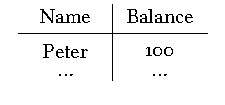
\includegraphics[width=\textwidth]
		{../illustrations/table.pdf}
	\caption{
		Active Record Example
	}
	\label{fig:table}
	\end{subfigure}
	%\quad
	\begin{subfigure}[t!]{0.67\textwidth}
	       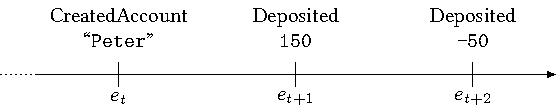
\includegraphics[width=\textwidth]
			{../illustrations/account-stream.pdf}
		\caption{
			Event Sourcing Example
		}
		\label{fig:log}
	\end{subfigure}
	\caption{Two different ways of storing the same current state.}
\end{figure}

\section{Active Record}
Many software systems require some kind of data management. A common approach
is to retain the current state of an application within some kind of data 
storage (e.g. a database) and return it on request. \emph{Active Record} is a 
software pattern which refers to the interaction with this current state (i.e. 
the active record) by applying create, read, update, or delete operations
(CRUD) on objects in a relational database (Figure \ref{fig:table}) 
\cite{Fowler2002}. 
In this approach, only the current state of an object is maintained and 
manipulated; previous values are overwritten and everything not saved is 
lost. This approach fits well for many applications but has shortcomings 
in terms of traceability and support for operations on the history.

\section{Event Sourcing}
\label{sec:es}
Most literature on event sourcing can be found online in blog posts, 
presentations, and software documentation. Academic literature on the 
topic is scarce.
This section provides an overview on how event sourcing is defined in
different resources and establishes the vocabulary used throughout this 
thesis.

\subsection{Different Definitions}
There is no standardized vocabulary on the topic, the terminology and 
definitions vary depending on the author. 

\paragraph{Martin Fowler}{
The term event sourcing was first established in a blog post by Martin 
Fowler \cite{Fowler2005} in 2005. 
He describes events as a series of changes in the state of an application. 
This series of events captures everything required to rebuild the current 
state. He views events as immutable and the event log as an append-only 
store. Events are never deleted, the only mean to revoke an event is a 
retroactive event~\cite{Fowler2005_2}. 
Once appended to the event log, this retroactive event acts as an inverse
event to a prior event and revokes its effects. 
%
Fowler does not distinguish clearly between events and the commands 
(i.e. actions) which triggered them.
This is an issue which is addressed in various works \cite{Chassaing2013, Reitzammer2013}.
}

\paragraph{Greg Young}{
Greg Young is another renowned author in the event sourcing domain. 
He describes event sourcing as ``storing [the] current state as a series of 
events and rebuilding state within the system by replaying that series of 
events'' \cite{Young2010}.
In his view, the event log possesses an append-only behavior as well: 
``[events] have already happened and cannot be undone'' \cite{Young2013}.
What Fowler calls retroactive events, Young describes as reversal
transactions \cite[p.31]{Young2013}.
}

\paragraph{Udi Dahan}{
Udi Dahan is a further author of a number of relevant blog posts and articles 
concerning event-sourced systems. To him, event sourcing refers to ``the state 
of the domain model being persisted as a stream of events rather than as a 
single snapshot [\dots]'' \cite{Betts2013}.
}

\paragraph{Martin Krasser}{
The articles and presentations by Martin Krasser concerning the persistence 
module in the Akka toolkit provide another view on event sourcing 
\mbox{\cite{Krasser2013, Krasser2015}.}
In this context, actors in a distributed system communicate via messages, 
which trigger state changes. Event sourcing is used as the mean to persist 
changes to the state of an actor.
State changes are ``appended as immutable facts to a journal'' \cite{Krasser2013}. 
A motivation for using it is that this approach ``allows for very high 
transaction rates and efficient replication''.
Recovering the state of an actor (e.g. after a restart or crash) is done by 
reapplying (i.e. replaying) the persisted events.
}


\ \\
The common ground of all these definitions is to publish every change to the 
state of an object (or system, or application) as an immutable event to an 
append-only event log. 
This results in a series of events, which when replayed always leads to the 
exact same state of the object (Figure \ref{fig:log}). Individual definitions 
vary or make no statement in terms of the editing semantics of the event log, 
the granularity of events, and the motivation for using it.

Where traditional architectures retain and maintain only the current state
of an object, event sourcing maintains all state-altering operations. Where 
CRUD offers four operations to apply modifications, event-sourced systems 
are restrained to only one operation: append-only.

\subsection{Benefits of Event Sourcing}
\label{sec:es-cs-benefits} 
An often found recommendation in literature is to apply event sourcing only in 
a clearly delimited part of a system and not force its usage upon a context 
where it does not appear beneficial \cite{Betts2013}.
A commonality often found in event-sourced systems, is that they possess a 
complex business logic. This is opposed to e.g. an application that provides 
``just'' an editing frontend to a relational database. We now briefly describe 
some of the benefits which an event-sourced architecture can provide.

\paragraph{Audit Log}{
In regulated areas (e.g. the financial industry), government regulations in 
many countries require companies to maintain records on the operation of a 
system. For example, the governmental regulations in the United States require 
brokers to keep their records in a non-rewriteable, non-erasable format \cite{sec17a}.
Event sourcing, with its append-only event log and immutable event characteristic, 
fits this requirement very well. Technologies such as write-once-read-many (WORM) 
data storages can be used complementarily with event sourcing.
If a WORM storage is used, the device prevents alterations of data in the hardware 
and allows only the appending of new data. 
}

\paragraph{Debugging}{
The captured events can be used to gain further insights into how the system 
reached its current states and which events were responsible for it. This is 
a strength in terms of traceability and debugging capabilities, since it makes 
it easier e.g. to retrace where a bug originated in a system.
}

\paragraph{Scalability}{
The append-only nature of an event log is thought to be beneficial for scalable 
architectures.
%
In such architectures it is common to have multiple replicated instances of the
same data model. These replications need to be kept in synchronization, in order 
to provide a consistent view on the data.
In event-sourced systems, the appending of events is the only mean to synchronize 
the replicated instances.
Due to fewer necessary locks, an append-only architecture with immutable events 
is thought to scale easier for reads than e.g. an architecture with a need for 
model synchronization via updates \cite[p.14-15]{Anderson2010}\cite{esdocs}.
}

\paragraph{Informative Value}{
Another motivation for applying event sourcing can be the informative value
(also sometimes referred to as ``business value''\footnote[1]{\href{http://docs.geteventstore.com/introduction/event-sourcing-basics/\#business-value-of-the-event-log}{http://docs.geteventstore.com/introduction/event-sourcing-basics/\#business-value-of-the-event-log}
}) of retrospectively examining the event log. All past states of a system 
can be reconstructed or queried. 
This can provide great value to systems, especially when the analysis of 
interaction with the system (e.g. customer behavior) is important. In such 
systems it is usually unknown what analysis one will execute in the future.
An example to illustrate this is an online shop where a shop administrator 
wants to list all products which have at some point been removed from a 
shopping cart. In event-sourced architectures, the state of the shopping 
cart at each past point can be queried.
}

\ \\
There are a number of documents describing how event sourcing has been applied 
in real-world systems. To highlight two information-rich documentations:
The financial trading platform LMAX utilizes event sourcing \cite{Fowler2011}
and a documentation published by the Microsoft Windows Azure team describes several 
case studies \cite{Betts2013}.
Furthermore, event-sourced frameworks like Akka\footnote[2]{\href{http://akka.io/}{http://akka.io/}}, 
Event Store\footnote[3]{\href{https://geteventstore.com/}{https://geteventstore.com/}}, or the Eventuate\footnote[4]{\href{https://rbmhtechnology.github.io/eventuate/}{https://rbmhtechnology.github.io/eventuate/}} 
toolkit by the Red Bull Media House provide the foundation for a number of 
real-world systems. 
 
\subsection{Thesis Terminology}
\label{sec:thesis-vocabulary}
Now that various authors' understanding of event sourcing has been described,
we establish the terminology used throughout this thesis. Since authors in the 
field use varying terminology, our terminology may differ from the individual 
authors' understanding.

\paragraph{Event}{
An event is a change to the state of an application. Each event is appended to 
the event log. It is important to note that the state change has already 
occurred to the entity. 
To reflect this, we name events as verbs in the past tense (e.g. \evt{ProductCreated}).
The granularity of events is defined through the context in which event sourcing 
is applied.
%
Events can be replayed in order to rebuild the state of a system up to a 
certain point. Except for the first event, each event builds upon the previous 
event. A replay process always needs to start from the beginning, though 
snapshots may be used as substitutions. 
}

\paragraph{Snapshot}
Snapshots are an established mean to optimize the process of restoring state. 
They represent the state of the system at a certain point in the event log 
and can be used instead of replaying the events prior to the snapshot.

\paragraph{Event Log}{
The event log provides the stream of all events which belong to an application.
An exchangeable term for the event log is the \emph{event stream}.
Figure \ref{fig:projections} depicts an excerpt of a hypothetical event log.

\begin{figure}[h!]
	\centering
	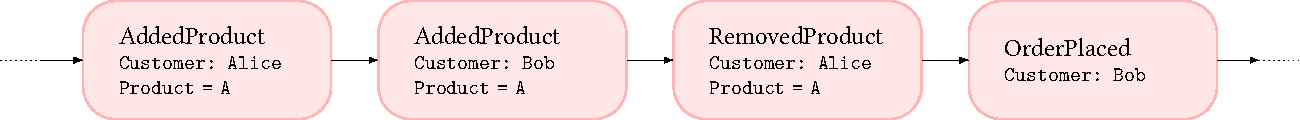
\includegraphics[width=1.0\textwidth]
		{../illustrations/projections2.pdf}

	\caption{
		An excerpt from a hypothetical event log in an online shop.
	}
	\label{fig:projections}
\end{figure}
}

\paragraph{Command}{
In the context of this thesis, a command resembles a requested change to an 
application. A command always results in an event, even in case of a failure.
Commands are typically named in the imperative form (e.g. \cmd{CreateProduct}).
}

\paragraph{Retrospection}
We use the term \emph{retrospection}, to describe the passive (i.e. read-only) 
access of a system's history and prior states.

\paragraph{Retroactive Computing}
With \emph{retroactive computing} (or \emph{retroaction}), we describe the 
interaction with an application's history.  %we describe the active (i.e. writing) 
This includes applying passive retrospective operations, as well as actively
modifying a history. Modifications can be applied through removal or insertion 
operations, as well as a retroactive change of the underlying application 
logic (the source code). This is examined in further detail in Chapters 
\ref{chp:concept} and \ref{chp:programming}.
